\documentclass[times,11pt]{ACME2015article}
\usepackage{amsmath,amssymb,amsthm,mathrsfs,graphicx}
\usepackage{natbib,subfigure}
\usepackage{titlesec}
\usepackage{color}
\usepackage{bm}
\usepackage{graphicx}
\usepackage{caption}
\usepackage{subcaption}

\setlength{\parindent}{0pt}
\setlength{\parskip}{5pt plus 2pt minus 1 pt}

\topmargin  -25mm
\evensidemargin 0mm
\oddsidemargin  0mm
\textwidth  160mm
\textheight 267mm
%\renewcommand{\baselinestretch}{1.0}
\frenchspacing
\sloppy
\titlespacing{\section}{0pt}{\parskip}{0.01\parskip}
%%%%%%%%%%%%%%%%%%%%%%%%%%%%%%%%%%%%%%%%%%%%%%%%%%%%%%%%%%%%%%%%%%%%%%%
\newcommand{\mb}[1]{\boldsymbol{#1}}
\newcommand{\E}{\mb{E}}
\newcommand{\B}{\mb{B}}
\newcommand{\EMH}{\mb{H}}
\newcommand{\D}{\mb{D}}
\newcommand{\F}{\mb{F}}
\newcommand{\weightfunc}{\mb{W}}
\newcommand{\R}{\mb{R}}
\newcommand{\pder}[2][]{\frac{\partial#1}{\partial#2}}
\newcommand{\pdert}[1]{\frac{\partial#1}{\partial t}}
\newcommand{\figref}[1]{figure \ref{#1}}
\newcommand{\ut}{\frac{\partial \mb{U}}{\partial t}}
\newcommand{\fk}{\frac{\partial \mb{F_k (\mb{U})} }{\partial x_k}}


\begin{document}
\pagestyle{empty}

\begin{flushright}
{\fontsize{8}{10}
\it Proceedings of the 23$^\mathrm{rd}$ UK Conference of the\\
Association for Computational Mechanics in Engineering\\
8 - 10 April 2015, Swansea University, Swansea\\} \vskip 1.2 cm
\end{flushright}

\begin{center}
{\fontsize{14}{20}\bf Computation of resonant modes in cavities with a Discontinuous Galerkin time domain approach
}\end{center}


\begin{center}
\textbf{M. Dawson, R. Sevilla, O. Hassan and K. Morgan}\\
\end{center}

\begin{center}
{\fontsize{10}{12}
Zienkiewicz Centre for Computational Engineering, College of Engineering, Swansea University, Swansea, Wales, UK SA2 8PP\\
}\end{center}

\begin{center}
\{743587,R.Sevilla,O.Hassan,K.Morgan\}@swansea.ac.uk\\
\end{center}
%
\begin{center}
\textbf{ABSTRACT}\\[1mm]
\end{center}
%

\begin{normalsize}
.\newline
.\newline
.\newline
.\newline
.\newline

\textbf{\textit{Key Words:}} {\it Finite Element, Discontinuous Galerkin, Electromagnetics, Resonant Cavities, Time Domain }
%
\\
\section{Introduction}
Recent advances in manufacturing techniques, such as electron beam lithography, make it possible to manufacture resonators on the scale of the wavelength of light. It has been demonstrated that such devices have well defined resonances and high quality factors. However, the typical scale and the geometric complexity introduce several challenges for numerical simulation.

Behaviour of these resonators is described by Maxwell's equations of classical electromagnetics. For metallic devices, the frequency dependence of material parameters, known as dispersion, is accounted using the Drude models. Frequency domain solvers \cite{ref1} are traditionally employed to find the resonant frequencies and associated modes, but as the scale and geometric complexity of the devices increases, the large eigenvalue system that must be solved becomes computationally prohibitive.

We propose to use the Discontinuous Galerkin (DG) method with explicit time marching, which only requires solving a block diagonal system of equations for each time step \cite{ref2}. The resonant frequencies, quality factors and mode shapes can then be recovered by a fourier transform of the time domain solution.

\section{Methodology}
%\subsection{Time Domain}
The behaviour of nano-scale resonators can be simulated using the Maxwells equations of classical electromagnetics. For metallic devices an additional coupled Auxiliary Differential Equation (ADE) is required to accounts for the frequency dependence of the material parameters due to finite time required for materials to respond to applied fields using the Drude model of solids. The system of equations to be solved can be written in linear, dimensionless conservation form as

\begin{equation}\label{maxwell-eqtns}
\pder[\mb{U}]{t} + \sum^{nsd}_{k=1} \pder[\mb{F}_k(\mb{U})]{x_k} = \mb{S}(\mb{U})
\end{equation}

where nsd denotes the number of spatial dimensions. The vector of unknowns, $\bm{U}$, and the flux vectors, $\bm{F_k}$, are given by

\begin{equation}\label{mypaper_eqn:sample_eqation}
\begin{array}{ccccc}
\mb{U} = \begin{pmatrix} \epsilon E_1 \\ \epsilon E_2 \\ \epsilon E_3 \\ \mu H_1 \\ \mu H_2 \\\mu H_3 \\ J_1 \\ J_2 \\ J_3 \end{pmatrix}
&
\mb{F_1} = \begin{pmatrix}0 \\ H_3 \\ - H_2 \\ 0 \\ - E_3 \\ E_2 \\ 0 \\ 0 \\ 0 \end{pmatrix}
&
\mb{F_2} = \begin{pmatrix} -H_3 \\ 0 \\ H_1 \\ E_3 \\ 0 \\ - E_1 \\ 0 \\ 0 \\ 0 \end{pmatrix}
&
\mb{F_3} = \begin{pmatrix} H_2 \\ -H_1 \\ 0 \\ -E_2 \\ E_1 \\ 0 \\ 0 \\ 0 \\ 0 \end{pmatrix}
&
\mb{S} = \begin{pmatrix} 0 \\ 0 \\ 0 \\ 0 \\ 0 \\ 0 \\ \omega_d^2 E_1 - \gamma_d J_1 \\ \omega_d^2 E_2 - \gamma_d J_2 \\ \omega_d^2 E_3 - \gamma_d J_3 \end{pmatrix}
\end{array}
\end{equation}

where $E_k$, $H_k$ and $J_k$ are the $k$th spatial components of the dimensionless intensity vectors of eletric field and magnetic field and material polarisation current respectively. For 2-dimensional problems the system of equations in Equation \ref{maxwell-eqtns} decouples into two independent systems of three unknowns: the transverse electric (TE) and transverse magnetic (TM) modes.

We propose to use the DG time domain method with explicit time marching. The domain $\Omega$ is discretised by an unstructured mesh and Equation \ref{maxwell-eqtns} may be expressed in weak DG form on an element $\Omega_e$ as

\begin{equation}\label{dg-weak-form}
\int_{\Omega_e} \mb{W} \frac{\partial \mb{U}_e}{\partial t} d\Omega  + \int_{\Omega_e} \mb{W} \cdot \left(  \sum_k \frac{\partial \mb{F}_k(\mb{U}_e)}{\partial x_k} -  \mb{S}(\mb{U}_e) \right) d\Omega + \int_{\partial \Omega_e} \mb{W} \cdot \mb{A}_n^{-} \llbracket \mb{U}_e \rrbracket d\Gamma = 0
\end{equation}

where $\bm{U}_e$ denotes the solution vector restricted to the element $\Omega_e$, $\bm{W}$ is a test function,  $\llbracket \bm{U}_e \rrbracket = \bm{U}_e 􏰇- \bm{U}^{out}$ denotes the jump of the solution across the element boundary $\Gamma_e$. The following form, derived from an upwind approximation, is used to evaluate the boundary term [\ref{flux-reference}] (** do I need to be more specific on the numerical flux?? ** )

\begin{equation}
\mb{A}_n^{-} \llbracket \mb{U}_e \rrbracket = \frac{1}{2}
  \begin{pmatrix}
    - \mb{n} \times \llbracket \mb{H} \rrbracket  + \mb{n} \times ( \mb{n} \times \llbracket \mb{E} \rrbracket ) \\
    \mb{n} \times \llbracket \mb{E} \rrbracket  + \mb{n} \times ( \mb{n} \times \llbracket \mb{H} \rrbracket )
  \end{pmatrix}
\end{equation}

The DG weak form given in Equation \ref{dg-weak-form} on each element leads to a system of ordinary differential equations

\begin{equation}\label{eqtn-sys}
\mb{M} \frac{ d\mb{U}}{dt} + \mb{R}(\mb{U}) = 0
\end{equation}

where $\mb{U}$ is the vector of nodal values, $\mb{M}$ is the mass matrix and $\mb{R}(\mb{U})$ is the residual vector. Note that solving the system given by Equation \ref{eqtn-sys} requires solving a block diagonal system only for each time step. 

%\subsection{Frequencies Domain}

\begin{figure}[htbp!]
 \centering
 \includegraphics[width=\textwidth]{Figures/SpectrumSchematic}
 \caption{Schematic of frequency finding process. Left: the excitation of a rectangular 2D cavity by a gaussian initial condition. Centre: a short sample of the solution sampled at a point in the domain at each time step. Right: The spectrum obtained following a Fast Fourier Transform showing well defined peaks at the resonant frequencies. The green lines indicate the analytical values of resonant frequencies. }
 \label{frequency_schematic}
\end{figure}

Quantities of interest for a resonator are the eigenspectrum, resonant frequencies and the mode shapes of the electric field. In order to obtain the eigenspectrum the cavity is excited and the solution allowed to evolve for a given time period, $T$. The cavity excitation could be simply an initial condition such as a dirac delta or gaussian function centered on a point in the domain, although more complicated strategies are available [reference?]. We capture a signal by sampling the solution at a point at every time step and use a Fast Fourier transform or similar, more sophisticated, techniques to obtain an eigenspectrum. The resolution of the spectrum obtained is limited by

\begin{equation}\label{spec-resolution-eqtn}
don't - have - equation - resolution - in - terms - of - T
\end{equation}

and the highest frequency captured is limited by

\begin{equation}
don't - have - equation - resolution - in - terms - of - dt
\end{equation}

The resonant frequencies is then the location of peaks in the eigenspectrum, which can be obtained by curve fitting. It is clear that the accuracy of the resonant frequencies obtained depends on the length of signal obtained - so a longer run of the simulation is desirable. Other more advanced techniques such as the Filter Diagonalisation Method can also be used to obtain the resonant frequencies directly from the sampled signal with greater accuracy for a given signal. Once a resonant frequency is known, the associated mode shape can be calculated by re-running the DG simulation [[ ** should I have more detail here? would be nice to say this without using too much space/detail ** ]]

Since resolution of the frequency spectrum obtained is determined by the period $T$ for which the solution is known, the ease of parallelisation of the DG method is particularly attractive to allow the sampling of a signal of the required duration in reasonable computational time.

\section{Results}

%\subsection{Free Space Cavity}

The first example presented is a rectangular 2D non-dispersive free-space cavity (i.e. $\epsilon_r = \sigma_r = 1$, $\omega_d = \gamma_d = 0$) with a width twice its length, surrounded by a perfect electric conductor (PEC). The inital condition constituted a gaussian function %centered at a point (0.19, 0.034)
and the solution was monitored at another point. % (0.4,-0.3)
The problem was selected for validation as analytically expressions for the resonant frequencies fo this cavity are known [reference]. Figure \ref{freeSpaceConvergence} shows the error in the frequencies calculated by simulation as compared to the known frequencies decreasing with signal period $T$ as expected from Equation \ref{spec-resolution-eqtn}.

%0.19141 0.034593 500
%-0.71722 -0.31595 500
%0.043817 0.35284 500
%0.70799 0.34823 500
%-0.1499 -0.26982 500
%0.55117 -0.13145 500
%-0.52811 0.16374 500

\begin{figure}[htbp!]
 \centering
 \includegraphics[height=7cm]{Figures/FDMEvolutionWithPeriod/FDM_p1_U5_freq3_edited}
 \caption{Convergence of the calculated resonant frequencies to the known analytical solutions as the period T is increased for different mesh refinement in a free space cavity.}
 \label{freeSpaceConvergence}
\end{figure}

%\begin{wrapfigure}{r}{0.4\textwidth}
% \centering
% \includegraphics[width=0.35\textwidth]{Figures/FDMEvolutionWithPeriod/FDM_p1_U5_freq3_edited}
% \caption{Convergence of the calculated resonant frequencies to the known analytical solutions as the period T is increased for different mesh refinement in a free space cavity.}
% \label{freeSpaceConvergence}
%\end{wrapfigure}

%\subsection{Dispersive Cavity}

In metallic resonant cavities of interest dispersive effect cannot be neglected. The implemetation of a dispersive medium was validated by solving Maxwells' equations (Equation \ref{maxwell-eqtns}) with an additional volumetric source added to the right hand side such that the problem had an exact known solution. The same 2D rectangular cavity as the free-space example was used but filled with a gold medium ($\epsilon_r = 1, \sigma_r = 1, \omega_d = , \gamma_d = $ ).
%inputData%plasmaFreq(1) = 6.743333333333332291D0,
%inputData%mat_gamma(1) = 0.079899999999999999D0,
The solutions obtained and the $L^2(\Omega)$ norm error in the solution are shown in Figures \ref{dispersive_validation} and \ref{dispersive-cavity-error} respectively.

%\begin{figure}[htbp]
% \centering
% \includegraphics[width=0.25\textwidth]{DispersiveCavityPlotU1}
% \includegraphics[width=0.25\textwidth]{DispersiveCavityPlotU2}
% \includegraphics[width=0.25\textwidth]{DispersiveCavityPlotU3}
% \caption{ Components $E_1$, $E_2$ and $H_3$ (TE mode) of the solution obtained for a rectangular cavity with a dispersive material and a volumetric source}
% \label{dispersive-cavity-error}
%\end{figure}
%
%\begin{figure}[htbp]
% \centering
% 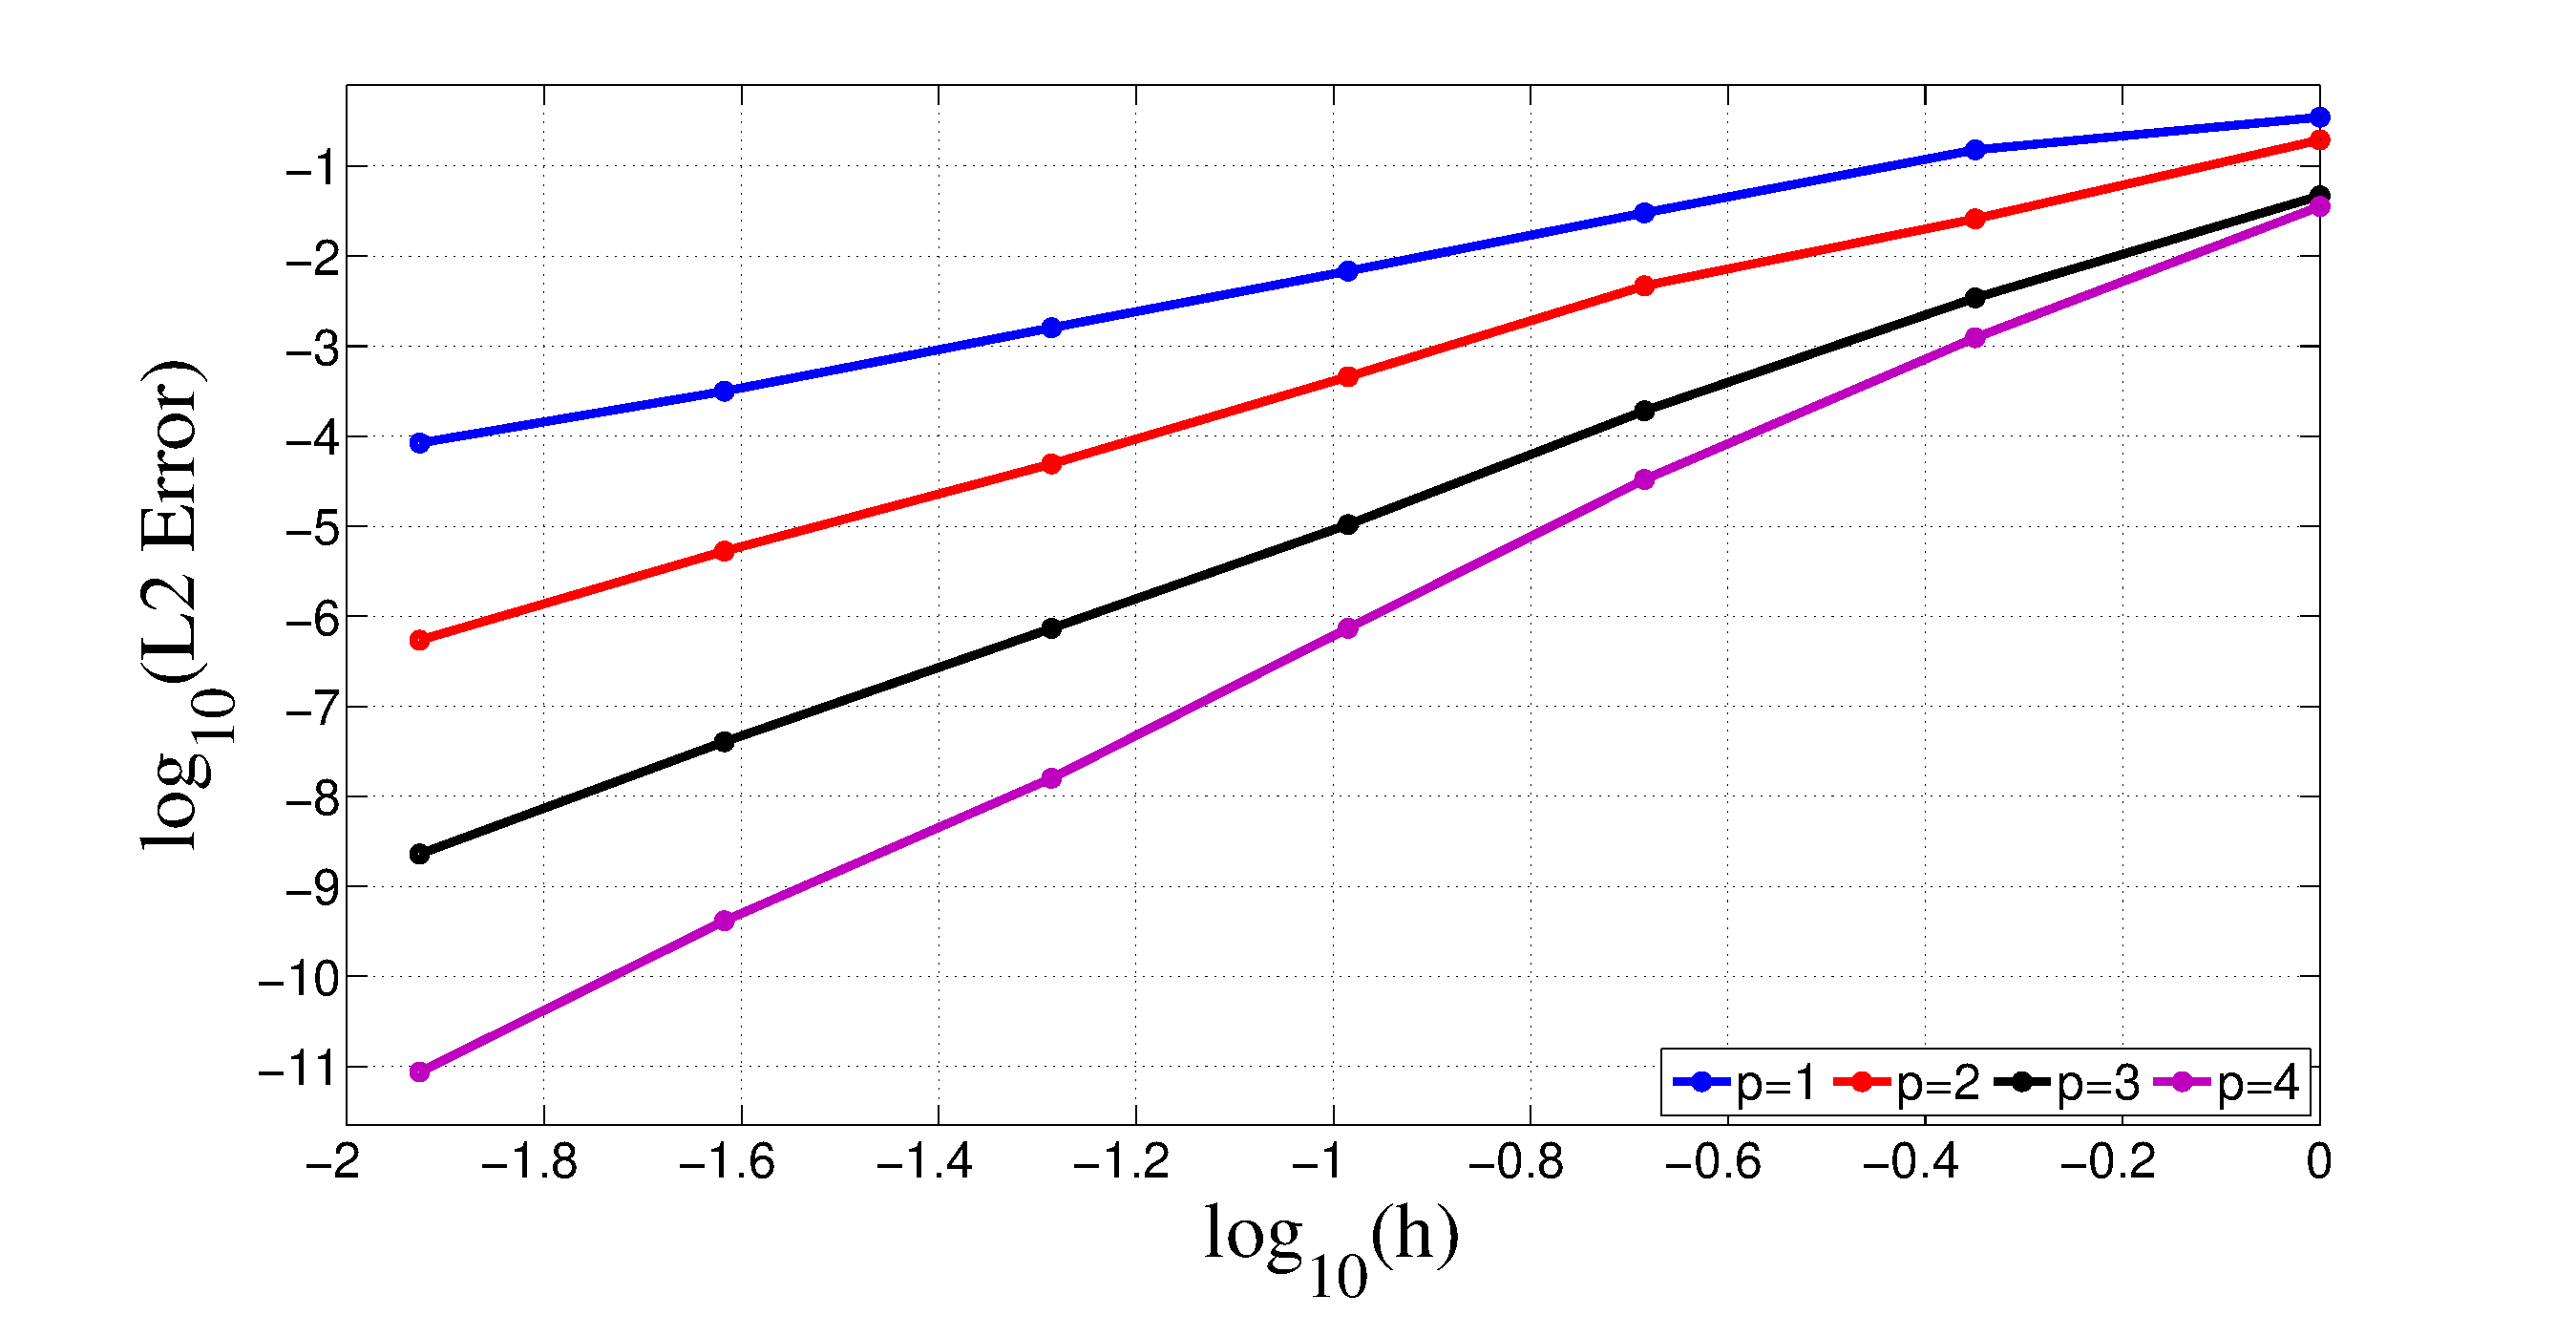
\includegraphics[height=7cm]{Figures/DispersiveValidationCase/convergenceAllComponents/L2vsH_TE_edited}
% \caption{h-convergence of the $L^2(\Omega)$ norm of the relative error in H1 for a cavity filled with dispersive material with a volumetric source term}
% \label{dispersive_validation}
%\end{figure}

\begin{figure}[htbp]
 \centering
 \includegraphics[height=7cm]{DispersiveCavityPlotU1}
 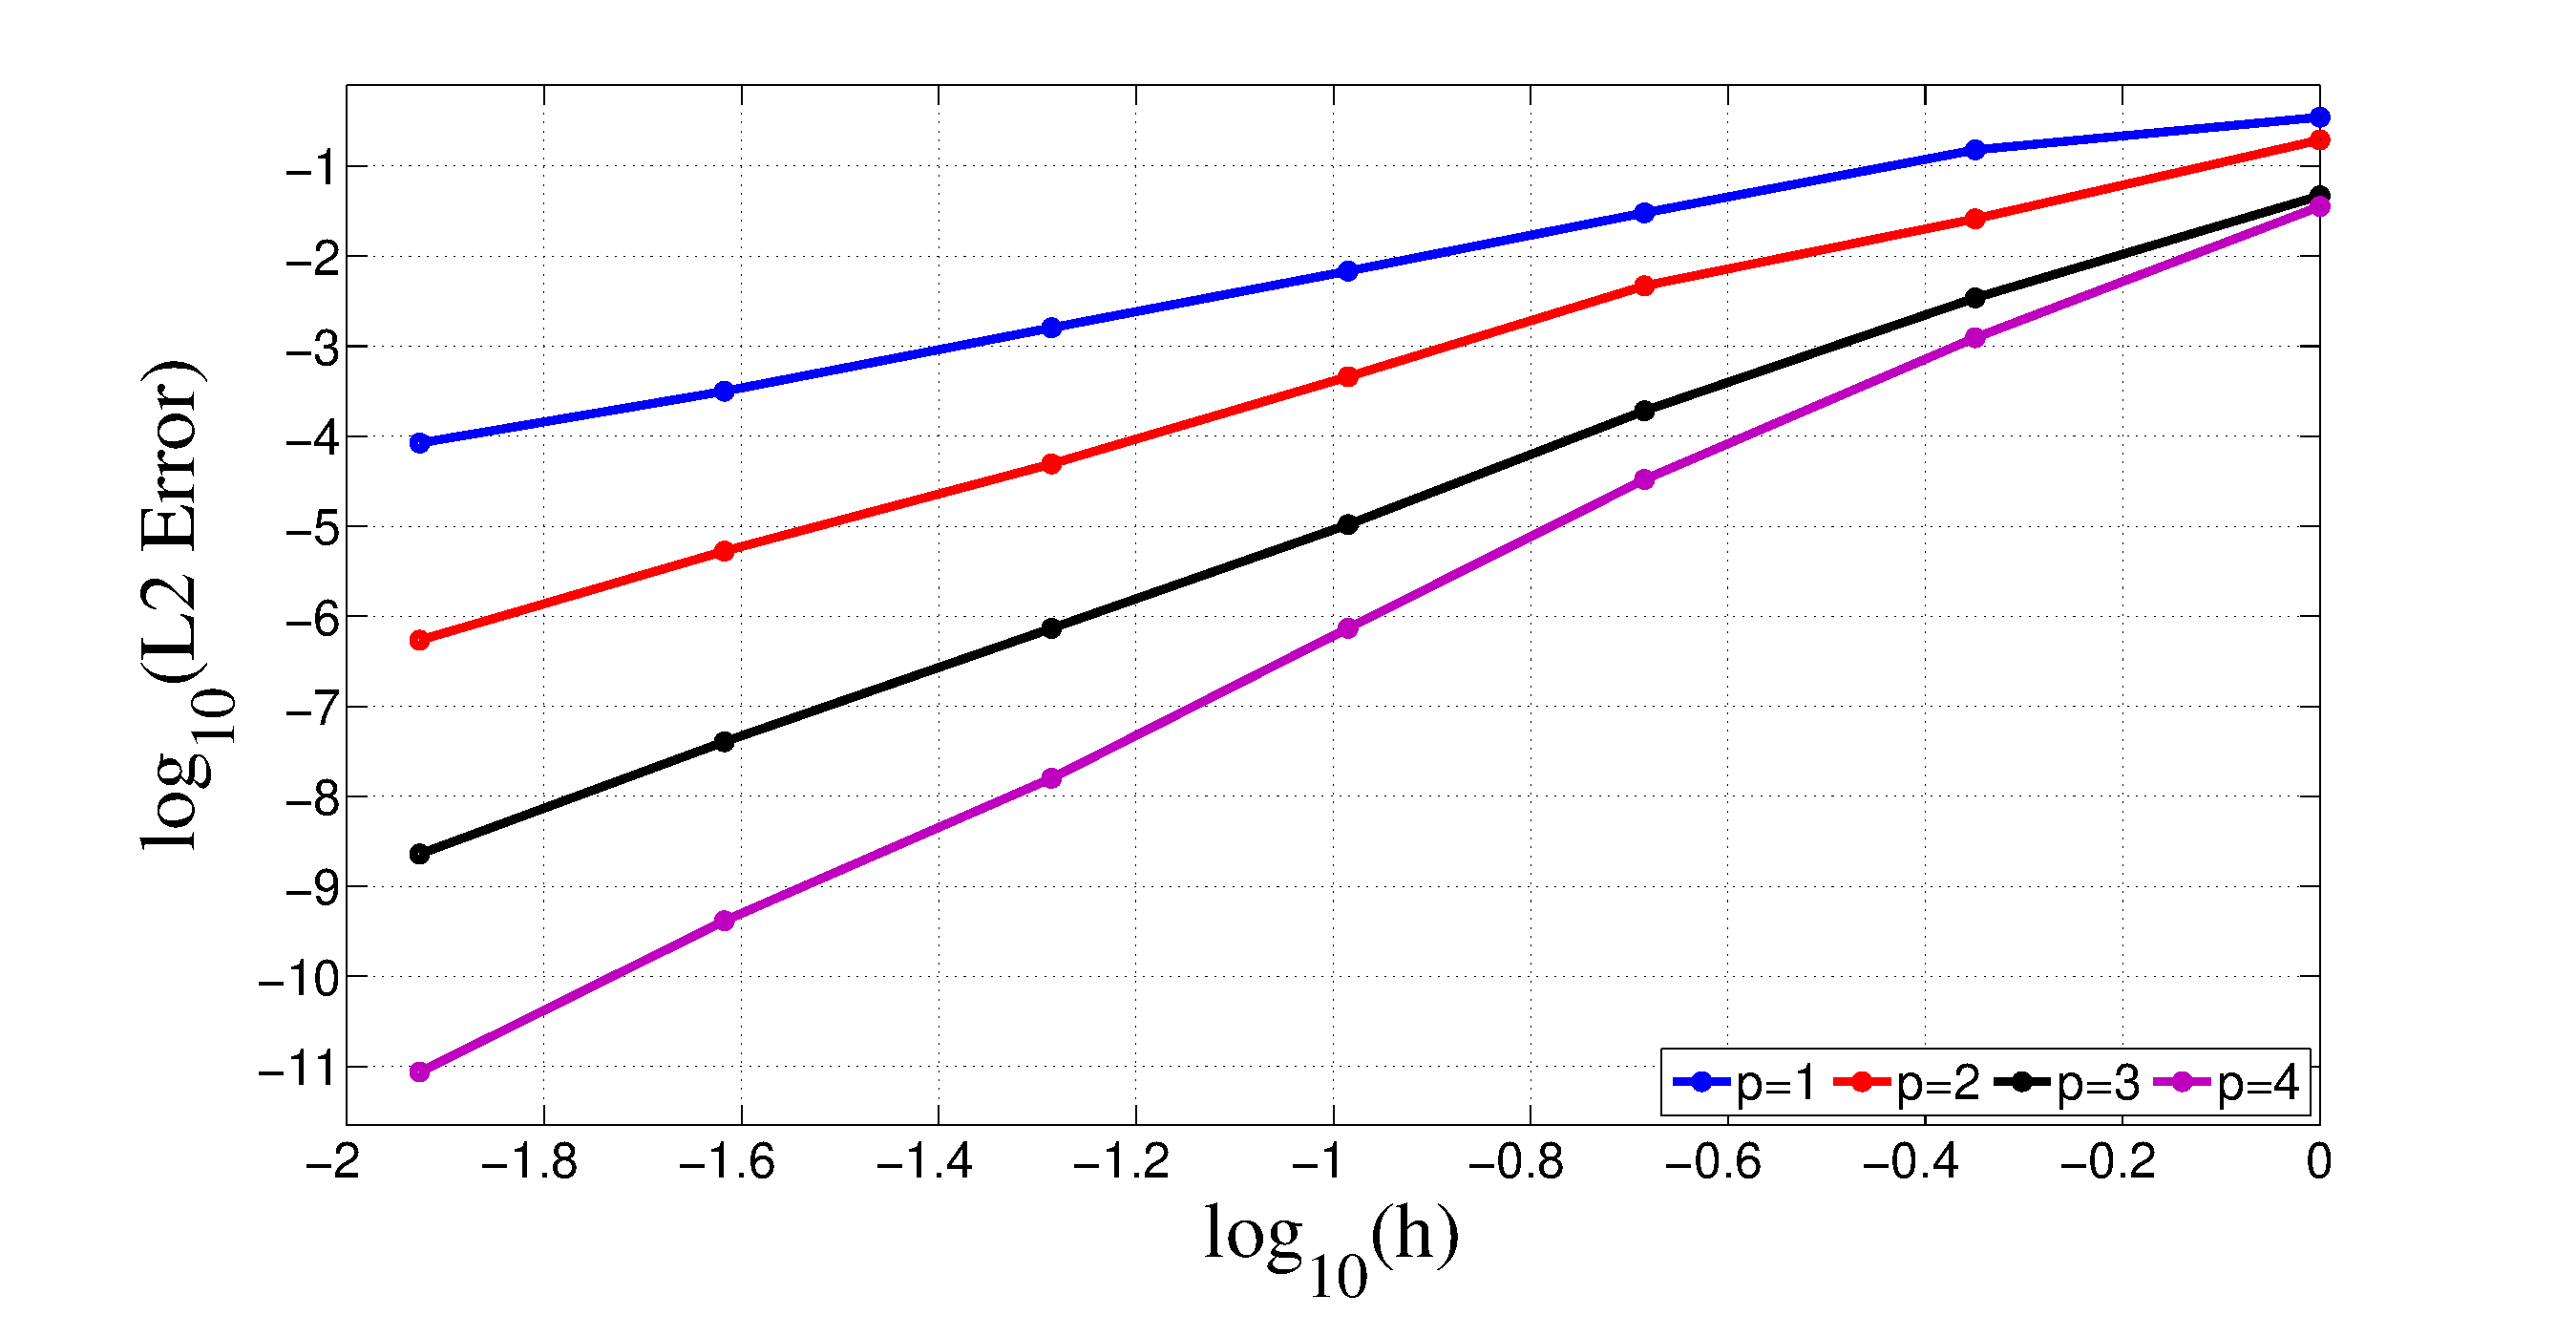
\includegraphics[height=7cm]{Figures/DispersiveValidationCase/convergenceAllComponents/L2vsH_TE_edited}
 \caption{Left: Components $E_1$, $E_2$ and $H_3$ (TE mode) of the solution obtained for a rectangular cavity with a dispersive material and a volumetric source. Right: h-convergence of the $L^2(\Omega)$ norm of the relative error in H1 for a cavity filled with dispersive material with a volumetric source term}
 \label{dispersive_validation}
\end{figure}

%\section{Achieving Frequency Resolution}

% Parallisation of the DG method can be attained with relative ease and allows the compution the evolution of the signal for an extended period of time.

%Parallisation of the DG code can be achieved by partitioning the physical domain into regions of adjacent elements with each processor performing computations on elements in a given region only. Since in the DG method calculations along faces involve values obtained from adjoining elements the values of the solution in neighbouring elements which are on other processors are communicated between each stage of the RK4 method.

% ** order of operations? - figure? ***

%The region calculated by each processor is selected to minimise the communication. Figure \ref{speed} shows the CPU time obtained as the number of nodes is increased.

% If communication was instantaneous we would expect doubling the number of processors to halve the computational time. In practice a limit is reached especially with smaller meshes where the communication dominates the behaviour and the additional speed up achieved by adding more processors is reduced. With smaller meshes this is especially true.

%\begin{figure}[htbp]
% \centering
% \includegraphics[height=7cm]{mypaper_example_graph}
% \caption{Cpu Times}
% \label{speed}
%\end{figure}
%
%Optimal convergence with mesh size was obtained for 3D parallelised code for high-order simulations with Pyramidal, Tetrahedral and *** elements and for 2D scattering from a circle with PML.

\section{Conclusions}
We discuss in detail the implementation of a parallelised DG electromagnetic solver, capable of full 3D simulation of dispersive metallic cavities. We present a study on the sampling rates and duration of the sampled signal required to obtain a given spectrum resolution. We validate the method by assessing the optical properties of resonators for problems with known solutions. Finally, we present results for a realistic metal-coated semiconductor nanocylinder resonator.


\section*{Acknowledgements}\label{mypaper_sec:acknowledgements}
The authors gratefully acknowledge the financial support provided by the S\^{e}r Cymru National Research Network in Advanced Engineering and Materials
\begin{thebibliography}{99}
\bibitem{bic}
N. Bicanic and O.C. Zienkiewicz. Constitutive model for concrete under dynamic loading. {\em Earthquake Engineering and Structural Dynamics}, 11, 689--710, 1983.

\bibitem{zie}
O.C. Zienkiewicz and R.C. Taylor. {\em The finite element method}, 4th. Edition, Vol. I, McGraw Hill, 1989.

\bibitem{zie}
W. M. Coombs, R. S. Crouch, C. E. Augarde, Unique critical state hyperplasticity, in: O. Laghrouche, A. EL Kacimi,P. Woodward, G. Medero (Eds.), {\em 19th UK Conference on Computational Mechanics (ACME-UK)}, pp.49–52, 2011.
\end{thebibliography}

\end{document}